% SPDX-License-Identifier: Apache-2.0
\section{From deployment value to financeable succession}
\subsection{A bounded continuation with fresh seeds}
The user's continuation asks how far the narrow deployment result can extend. It does not
replace any original experiment. Before fresh outcomes, we declared a 128-condition extension,
24 new seeds (3001--3024), the same 52-week horizon, \money{1,000} initial capital and
\money{200} reserve, with no replenishment. The \money{20} target is inherited from the
identified diagnostic slice; this is an explicitly selected-policy exploratory extension,
not a new primary test or a search over prices. Its complete freeze was publicly recorded
before execution \cite{successionfreeze}.

The main 48-cell grid crosses integration costs \money{0}/\money{2.50}/\money{5}/\money{10},
work arrival .1/.25/.5, deterministic/logit buyers and full-history/adoption-only accounting.
Eighty adverse corners test weekly upkeep of \money{2}/\money{5}, collection delays of
6/13 weeks, cheaper AI, cheaper humans, undercutting, a quality shock, failed initial integration
and dissatisfaction. Each intervention is specified at zero/\money{5} integration, .5 arrival,
both buyer rules and both cost bases. The failed-integration corner means immediate detection with a full charge and no forced
downtime; it does not represent a prolonged failed installation. Other calibration and the
core economic rules stay unchanged.
No horizon extension or relaxation of buyer preferences is allowed after outcomes.

The research envelope limits the new market run to 120 wall and CPU seconds and sets an
18:10:33 UTC research cutoff. Discovery is capped at three burdens and fifteen minutes;
at most one justified prototype could use twenty minutes of implementation and six fresh
confirmation missions across three arms. Unfinished work must be labeled unfinished.
Publication and custody work are separately recorded.

\subsection{A source-of-funds view without invented money}
Initial external funding does not itself disqualify a Flywheel. The question is whether later
productive activity generates resources that can finance another worthwhile asset without
repeated injections. Three accounts are therefore kept separate: prospective deployment,
full historical return and funding provenance.

The original strict earned-funds policy remains unchanged. A second read-only attribution
view deducts one reserve in the liquidity bound. Let \(H_t^{\rm seed}\) be only a verified
historical research bill paid from opening seed before any collections; \(U_t\) is an outstanding
generated-resource earmark not already accrued as expense. Then
\begin{equation}
G_t=\max\!\left[0,\,
\min(C_t-O_t-R,\ Y_t-E_t+H_t^{\rm seed})-U_t\right].
\label{eq:generated}
\end{equation}
Here \(Y_t\) is collected revenue and \(E_t\) all accrued expenses. Setup, first adoption,
delivery, failed integration, upkeep and refunds remain inside \(E_t\). Historical research
stays charged once in cash and full-return profit; it is excluded only from the prospective
operating-generation recovery subtotal. Unpaid or later research is never added back.
An earmark reduces both the cash and generation bounds, and is released when its bill accrues.
No actual second-asset commitment exists, so \(U_t=0\) in this study.

This convention identifies a funding ceiling, not an extra cash balance or a transfer.
The adoption-only end-of-year seed-2001 example has \money{122.65} in generated resources under
Equation~\ref{eq:generated}, while its original strict metric remains \money{-77.35}.
Its \money{200} liquidity reserve is protected in both views. A sensitivity also requires
historical research recovery in the generation bound.

The new discovery itself has unknown authoring/inference and human monetary cost. Denote this
incremental unpriced cost \(D\geq0\); it is not silently reclassified into the old historical bill
or treated as zero. Before new decisions alter a path, available funds after that discovery are
bounded above by \(\max(0,G_t-D)\), and its economic return falls by its attributed \(D\).
For paired arms the fixed-path effect becomes
\(\Delta_{BA}^{\rm after}=\Delta_{BA}^{\rm before}-(D_B-D_A)\);
unidentified differential discovery costs do not automatically cancel.
Reported \(G_t\) is consequently \emph{before this unpriced discovery}, not an all-in investment
budget. The complete cost of any candidate would have to fit the remaining amount.

\begin{figure}[H]
\centering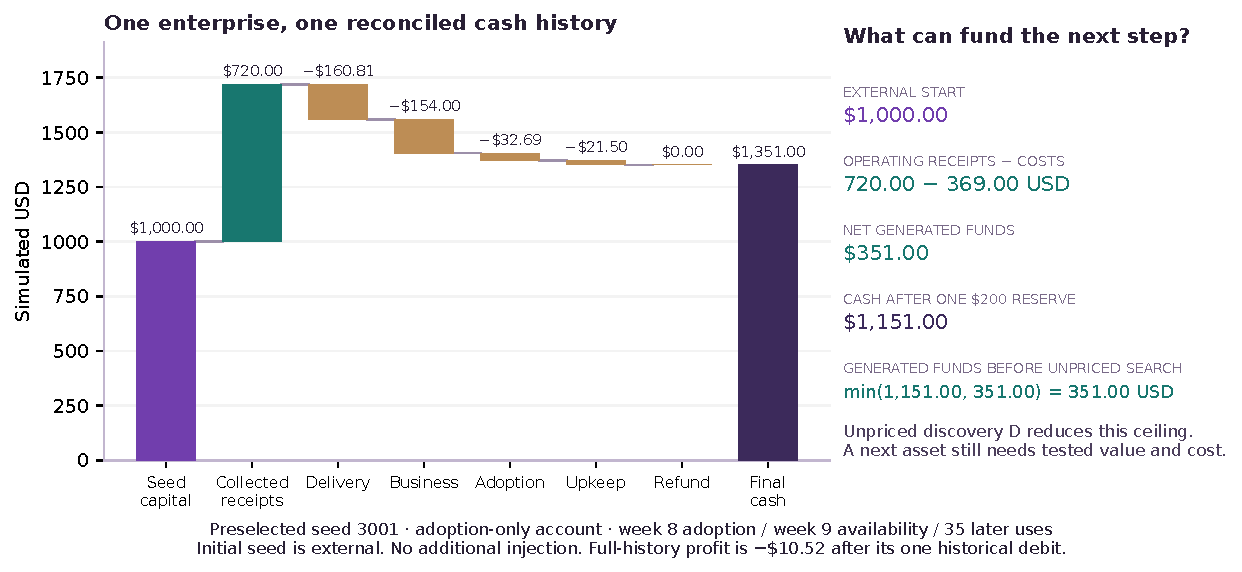
\includegraphics[width=\textwidth]{figures/finance.pdf}
\caption{Starting capital, productive collections, costs, reserves and the exact retained
investment in the connected fresh-seed path selected before extension outcomes. The provenance view exposes generated funds while
preserving the historical-return loss. The funding ceiling precedes the unpriced new discovery
cost \(D\); no hypothetical successor is purchased.}
\end{figure}

% SPDX-License-Identifier: Apache-2.0
\subsection{Fresh-seed outcomes and the viable region}
The registered extension completed all 3,072 paired worlds and 9,216 enterprise histories at
17:27:04 UTC, before the scientific cutoff. Its bounded invocation used 53.97 wall seconds and
60.52 child CPU seconds, below both 120-second limits. All 128 declared conditions are retained.
Every monetary result in this subsection precedes the unpriced incremental discovery cost \(D\).
This qualification applies to profit, paired effects and funding ceilings.

At the predeclared reference---\money{20}, zero integration, .5 arrival, logit choice and
seed-inclusive prospective adoption---mean B profit is \money{151.70}, with conditional
95\% Monte Carlo interval [\money{93.56}, \money{209.84}]. The paired gain is \money{173.67},
interval [\money{137.44}, \money{209.90}]. A's mean profit is \money{-21.97}. All 24 B paths
adopt, but three lose money. B profit ranges from \money{-140.33} to \money{474.62},
median \money{148.67}, sample standard deviation \money{145.32}. Paired gains range from
\money{0.31} to \money{338.21}, median \money{169.26}, standard deviation \money{90.55}.
Thus the fresh simulation retains a positive conditional mean deployment effect while exposing
downside absent from the original twelve-world slice.

Charging the same \money{361.52} historical allowance once changes reference mean B profit to
\money{-209.82} and its mean paired effect to \money{-187.85}; every reference paired effect
is then negative. Across all 64 full-history extension conditions, none has positive mean
B profit or positive mean B-minus-A. There are nevertheless 22 individual full-history worlds
with both a profit and a positive paired effect. These finite paths must not be erased, nor
treated as an estimated real-world success probability. Across the 64 prospective conditions,
18 have positive mean B profit and 47 have positive mean B-minus-A. B and C tie exactly throughout.

\begin{table}[H]
\centering\small
\caption{Fresh-seed main grid at .5 arrival. Prospective B profit and paired gain, before
unpriced discovery; 24 worlds per row. Parentheses give conditional 95\% Monte Carlo intervals.
Integration cost is buyer friction, not supplier revenue.}
\begin{tabularx}{\textwidth}{llYrr}
\toprule
Choice & Integration & Mean B profit (USD) & Mean B--A & Losses\\
\midrule
Logit & $0.00$ & $151.70\ (93.56,\ 209.84)$ & $173.67$ & 3/24\\
Logit & $2.50$ & $110.17\ (54.48,\ 165.85)$ & $147.42$ & 5/24\\
Logit & $5.00$ & $65.30\ (7.25,\ 123.36)$ & $114.24$ & 10/24\\
Logit & $10.00$ & $-23.69\ (-69.02,\ 21.64)$ & $59.71$ & 16/24\\
Deterministic & $0.00$ & $61.39\ (-54.65,\ 177.43)$ & $107.26$ & 13/24\\
Deterministic & $2.50$ & $-10.40\ (-90.35,\ 69.55)$ & $60.48$ & 16/24\\
Deterministic & $5.00$ & $-57.83\ (-111.96,\ -3.70)$ & $47.25$ & 18/24\\
Deterministic & $10.00$ & $-118.57\ (-144.41,\ -92.74)$ & $6.24$ & 23/24\\
\bottomrule
\end{tabularx}
\end{table}

In the logit grid, mean prospective profit changes sign between \money{5} and \money{10}
integration. The deterministic grid changes sign between \money{0} and \money{2.50}, and even
its zero-friction mean has a wide interval and a majority of losing paths. At .25 or .1 arrival,
no main-grid condition has positive mean B profit. These are sampled sign brackets, not fitted
exact break-even points, a universal monotonicity result or a license to extrapolate demand.
The assumed ten provider minutes remain essential unidentified input; fresh market seeds do not
turn an AI finalization-action count into measured human effort.

\begin{figure}[H]
\centering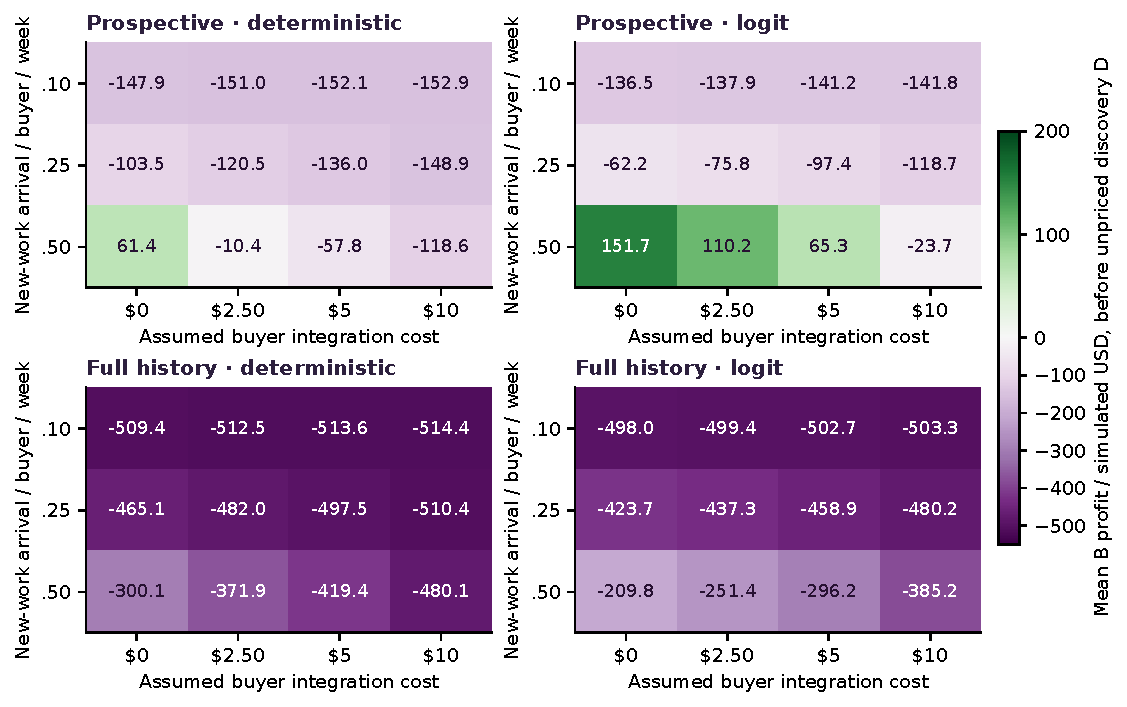
\includegraphics[width=\textwidth]{figures/succession-grid.pdf}
\caption{Every main extension cell, with the original horizon and capital. The prospective
region is sensitive to integration, recurrence and buyer-choice specification. Full-history
accounting remains separate. Values exclude the new unpriced discovery cost.}
\end{figure}

\begin{figure}[H]
\centering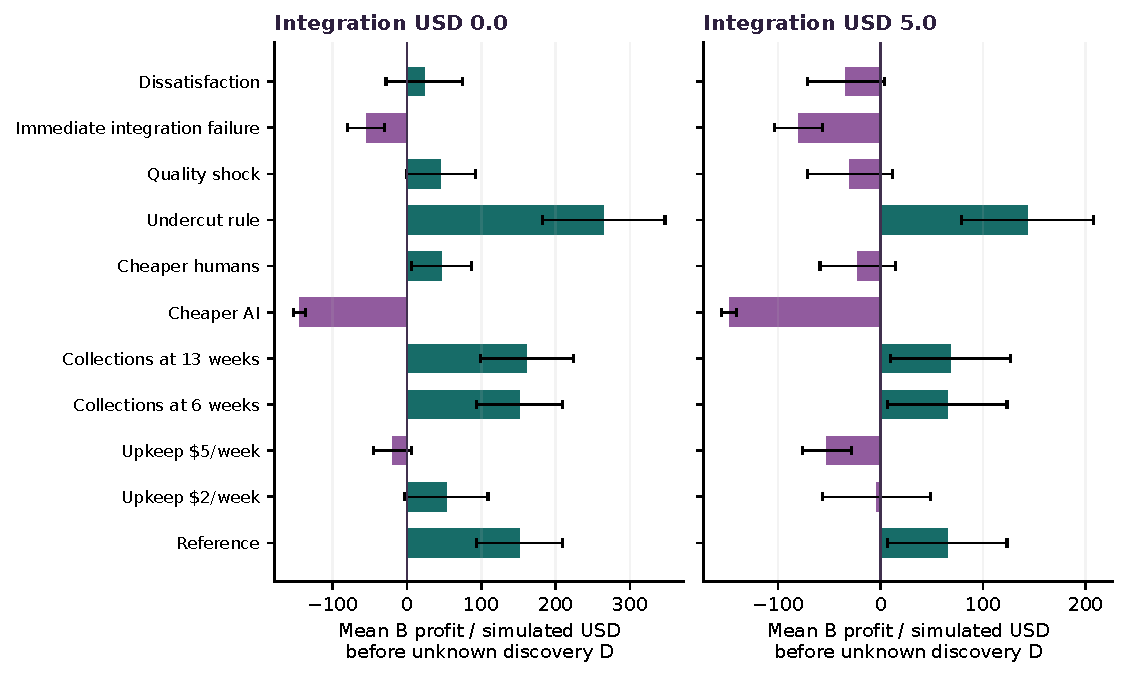
\includegraphics[width=\textwidth]{figures/succession-stress.pdf}
\caption{All ten predeclared perturbations and the reference for logit buyers at .5 arrival,
prospective accounting and zero/\money{5} integration. Intervals describe Monte Carlo variation,
not identified market parameters. A perturbation is not guaranteed to worsen outcomes under
every behavioral response. The complete table retains both buyer rules and both cost bases.}
\end{figure}

At zero integration, \money{2} weekly upkeep lowers mean B profit to \money{52.60};
\money{5} upkeep lowers it to \money{-19.85}. Cheaper AI removes deployment value:
mean profit is \money{-144.71} and mean B-minus-A is \money{-0.44}. Cheaper human provision
gives \money{46.31} mean profit, the quality shock \money{45.66}, and dissatisfaction
\money{23.40}; each becomes a negative mean at \money{5} integration.
Immediately detected failed integration produces \money{-54.66} profit and
\money{-32.69} incremental value at zero integration. It is a charged failure, not a free retry.

Collection timing alone does not necessarily reduce terminal profit when reserves cover the lag
and contracted receipts are drained. Six weeks reproduces the reference mean; thirteen weeks
gives \money{161.37}. Existing-event inspection finds 21/96 first buyer-choice divergences
across both integration levels and buyer rules; every one has unchanged quoted prices and a
human-provider cash gate that passes in the reference but binds under the longer delay.
For seed 3008 at week 35, a \money{67.50} delivery requirement fits \money{504.05} of reference
human-provider cash but exceeds \money{60.35} in the delayed path; that buyer switches to the
enterprise. No competitor insolvency occurs in these inspected cells.
Despite higher terminal mean B profit, the reference mean maximum during-service funding ceiling
falls from \money{153.04} to \money{69.68}. Payment timing can constrain succession before final
accounting catches up.

The undercut rule gives \money{264.54} mean profit because it sets the AI quote at \money{16},
whereas the adaptive reference reaches \money{7}--\money{17}. Fully 1,217 of 1,248 recorded
reference weekly quotes are below \money{16}; mean accepted AI jobs fall from 48.54 to 26.71,
and enterprise accepted jobs rise from 25.04 to 31.83. Undercutting the enterprise's \money{20}
is therefore weaker competition than many reference markdowns. These declared interventions
are not uniformly harsher conditions. The arithmetic inspection uses existing histories only;
it establishes a mechanism within this behavioral model, not a general benefit of delayed
payment, a favorable equilibrium or a real-world competitive advantage.

\subsection{Generated resources exist, but do not establish a second cycle}
The reference's mean terminal \(G\) is \money{162.29}, median \money{148.67}, range
\money{0}--\money{474.62}. Twenty-one of 24 paths have a positive terminal ceiling; twenty
have one during the productive year. This is a mean of nonnegative per-path ceilings, not
the mean profit of \money{151.70}. Charging historical research once does not automatically
erase operating generation: the cash bound still protects obligations and the reserve.
The stricter original prospective metric has mean \money{-48.30}.

The registered representative seed 3001 connects the entire sequence without selecting a
trajectory after outcomes. It has 321 changed-work opportunities, 249 supported, forty attempted
deliveries, 37 accepted and three rejected. Initial adoption costs \money{32.69} at week 8;
the exact first asset becomes available at week 9 and serves 35 later modeled jobs.
Gross invoices are \money{740}; \money{720} is collected and \money{20} defaults.
There are no refunds. Declared prospective costs total \money{369}: \money{154} business,
\money{160.81} delivery, \money{32.69} adoption and \money{21.50} upkeep.
Profit is \money{351}, cash \money{1,351}, and the paired gain \money{338.21}.
After the historical debit, profit is \money{-10.52}, cash \money{989.48} and paired gain
\money{-23.31}. The historical loss is visible even though the prospective operating-generation
ceiling is \money{351} under both cost bases.

This path first has a positive \(G\) at week 19; its maximum during the productive year is
\money{311}, followed by \money{351} after collections drain. The original strict metrics are
\money{151} prospective and \money{-210.52} full-history. These amounts cannot be spent before
they exist. No second asset is bought at any date.

For this path, a future investment could fit at most \(\max(0,351-D)\) dollars after the new
discovery, subject to its own timing, obligations and qualification. For the reference mean,
an attributed expected \(D_B\) reduces \money{151.70} of prospective profit dollar for dollar;
the paired benefit is also reduced by the differential cost \(D_B-D_A\). Neither cost is
identified. Accordingly, the study establishes a conditional supply of generated resources,
not all-in affordability or repayment of an unbuilt successor.


\subsection{The second-capability gate: no qualified purchase}
The bounded discovery examined three burdens in 321.8 elapsed seconds, not measured human labor.
Broader native application qualification is the most promising service direction: it could
extend a maintainer's component evidence into a fuller release decision. However, the current
61-case closure does not identify an authorized, reproducible broader contract, measured
remaining effort, complete cost bounds or a prospectively frozen fresh cohort.

Additional environment reuse already benefits all arms. The entire five-environment setup costs
19.894 CPU seconds, and changed tuples still require validation. No material extra attention
benefit is measured. Publication and accounting custody repairs are necessary research work,
but do not provide another productive capability for this component-assessment buyer.
The previously rejected baseline cache and existing importer owner's boundary remain intact.

The gate is therefore \textbf{NO-GO before construction}. There is no second implementation,
fresh second-asset confirmation, purchase, new customer job or claimed second-asset saving.
This does not say all future assets are worthless, and it does not erase the existing B/C
deployment value. The missing condition is a source-identified, worthwhile and tested next
asset whose complete cost fits generated funds after discovery, obligations and reserves.
Positive cash availability alone cannot supply that evidence.

\subsection{An evidence ladder}
\begin{table}[H]
\centering\small
\caption{Claims advance only as far as their evidence. Economic thresholds remain conditional
on declared scenarios and unidentified costs.}
\begin{tabularx}{\textwidth}{p{43mm}Y}
\toprule
Rung & Supported status\\
\midrule
Executed useful production & Established in the finite component scope: four fresh joint
questions, twelve complete assessments, actual reviewable decision packets.\\
Conditional deployment value & Positive within specified model conditions; preserved primary
failures and adverse outcomes remain visible. Original and fresh-seed results are separately labeled.\\
Full investment repayment & No tested full-history configuration has positive mean profit
or investment effect. Some individual paths do; actual all-in cost remains unknown.\\
Generated financing of a subsequent tested asset & Funding ceilings can be computed, but
no qualified second capability exists and its discovery cost is unpriced. A second cycle is not established.\\
Actual market receipts & Zero observed collections; no actual adoption is inferred from
simulated buyers or invoices.\\
Superior improvement process or self-acceleration & Not established. Conventional C ties B;
construction efficiency on comparable fresh problems has not been demonstrated.\\
\bottomrule
\end{tabularx}
\end{table}
